\documentclass[12pt]{article}
\usepackage{fullpage,geometry,amsmath,hyperref,graphicx,xcolor,amssymb,array,enumitem,minted}
\usepackage{indentfirst}
\usepackage[version=4]{mhchem}
\newcommand\norm[1]{\left\lVert#1\right\rVert}
\newcommand\normx[1]{\left\Vert#1\right\Vert}
\geometry{letterpaper,left=2.54cm,right=2.54cm,top=2.54cm,bottom=2.54cm}

\begin{document}
\begin{center}\Large\bf 
CS 357 - 04 Floating point representation\\
\end{center}
\begin{center}
Boyang Li (boyangl3)
\end{center}

\medskip
\noindent \textbf{Base-$\boldsymbol{\beta}$ system:} For a base-$\beta$ system, a number can be expressed as 
$$(a_n\dots a_{n-1} a_3 a_2 a_1 a_0 . b_1 b_2 b_3 b_4 \dots)_\beta = \sum_{k=0}^{n} a_k \beta^k +\sum_{k = 1}^{\infty} b_k \beta^{-k}$$

Commonly used system: Binary ($\beta = 2$), Octal ($\beta = 8$), Decimal ($\beta=10$) and Hexadecimal ($\beta=16$).

\medskip
\noindent \textbf{Convert integers between different systems:}
    \begin{itemize}
        \item \textbf{Base $n$ to decimal:} Use definition above.
        \item \textbf{Decimal to base-$n$:} Divide by $n$ until get quotient 0 and take the remainders in reverse direction.
    \end{itemize}

\medskip
\noindent \textbf{Convert decimals between different systems:}
    \begin{itemize}
        \item \textbf{Base $n$ to decimal:} Use definition above. There is a shortcut to convert the ``decimal" parts:
            \begin{enumerate}
                \item Convert the ``decimal" part into decimal (base-10) store the result in $a$
                \item The number of ``decimal" digits is $m$
                \item Calculate $\dfrac{a}{n^m}$, the result is the value of ``decimal" parts in the base-10 system.
            \end{enumerate}
        \item \textbf{Decimal to base-$n$:} Following the steps below:
            \begin{enumerate}
                \item Convert the integer to base-$n$ system.
                \item For the decimal part, multiplying by $n$
                \item Take the decimal part, repeat step 2 until get 0 in the decimal part.
                \item Now the base-$n$ number, we already get the integer part, the ``decimal" part are the \textbf{digits of integer part of each multiplication} in the forward sequence.
            \end{enumerate}
    \end{itemize}
    Example from textbook: Convert 23.375 to binary number.
    \begin{align*}
        23.375 &= (10111)_2 \\
        2 \cdot 0.375 &= 0.75 \\
        2 \cdot 0.75 &= 1.5 \\
        2 \cdot 0.50 &= 1.0
    \end{align*}
    
        So the final result is 23.375 = $(10111.011)_2$

        Note: Not all fractions can be expressed into a binary. Because you might get repeat result using the technique above. (Example: 0.1)

\newpage
\noindent \textbf{Floating point numbers:} Similar to scientific notation, the floating point number is usually binary. Here is the standard form:
    $$x = \pm q \cdot 2^m$$
    \begin{itemize}
        \item $\pm$ describes the sign
        \item $q$ is the \textbf{significand}
        \item $m$ is the exponent
    \end{itemize}

    Note: Usually we use the \textbf{normalized} floating number, where $1 \leq q < 2$.

\medskip
\noindent \textbf{Properties of normalized floating point:}
    $$x = \pm 1.b_1 b_2 b_3 \dots b_n \times 2^m = 1.f \times 2^m$$

    \begin{itemize}
        \item \textbf{Digits of fraction:} Either 0 or 1
        \item \textbf{Exponent range:} $m \in [L, U]$
        \item \textbf{Precision:} $p = n + 1$
        \item \textbf{Smallest positive normalized:} $2^L$
        \item \textbf{Largest positive normalized:} $2^{U+1} \left(1-\dfrac{1}{2^{n+1}} \right)$
    \end{itemize}

\medskip
\noindent \textbf{IEEE-754 standards:}
    \begin{center} \renewcommand\arraystretch{2}
        \begin{tabular}{|c|c|c|}
        \hline
           \textbf{Properties} & \textbf{IEEE-754 Single Precision} & \textbf{IEEE-754 Double Precision} \\
           \hline
           Number of bits & 32 & 64  \\
           \hline
           Size & 4 Bytes & 8 Bytes \\
           \hline
           Sign bit($s$) & Index 31 to the right (1 bit) & Index 63 to the right (1 bit)\\
           \hline
           Exponent bits($c$) & Index 30 - 23 to the right (8 bits) & Index 62 - 52 to the right (11 bits)\\
           \hline
           Fraction bits($f$) & Index 22 - 0 to the right (23 bits) & Index 51 - 0 to the right (52 bits)\\
           \hline
           Expression & $x = (-1)^s 1.f \times 2^m$ & $x = (-1)^s 1.f \times 2^m$\\
           \hline
           Exponent ($m$) & $c = m + 127$ & $c=m+1023$ \\
           \hline
           Mach. Epsilon ($\epsilon$) & $2^{-23}$& $2^{-52}$\\
           \hline 
           Smallest NFP ($UFL$) & $2^{-126}$ & $2^{-1022}$\\
           \hline
           Largest NFP ($OFL$) & $2^{128}(1 - 2^{-24})$ & $2^{1024}(1 - 2^{-53})$ \\
           \hline           
        \end{tabular}
    \end{center}
\newpage
\noindent \textbf{Corner cases of IEEE-754:} Here are some corner cases of IEEE-754.
    \begin{itemize}
        \item \textbf{Zero:} In our definition of floating point numbers above, we said that there is always a leading 1 assumed. This is true for most floating point numbers. A notable exception is zero. In order to store zero as a floating point number, we store all zeros for the exponent and all zeros for the fractional part. Note that there can be both +0 and -0 depending on the sign bit.
        \item \textbf{Infinity: }If a floating point calculation results in a number that is beyond the range of possible numbers in floating point, it is considered to be infinity. We store infinity with all ones in the exponent and all zeros in the fractional. $+\infty$ and $-\infty$ are distinguished by the sign bit.
        \item \textbf{NaN:} Arithmetic operations that result in something that is not a number are represented in floating point with all ones in the exponent and a non-zero fractional part.
    \end{itemize}

\medskip
\noindent \textbf{Machine Epsilon($\boldsymbol{\epsilon}$):} defined as the distance (gap) between 1 and the next largest floating point number.

\medskip
\noindent\textbf{Subnormal numbers:} However, we can go even smaller than this by removing the restriction that the first number of the significand must be a 1. These numbers are known as subnormal, and are stored with all zeros in the exponent. Technically, zero is also a subnormal number. \textbf{It is important to note that subnormal numbers do not have as many significant digits as normal numbers.}
\begin{center} \renewcommand\arraystretch{2}
        \begin{tabular}{|c|c|c|}
        \hline
           \textbf{Properties} & \textbf{IEEE-754 Single Precision} & \textbf{IEEE-754 Double Precision} \\
           \hline
           Exponent bits($c$) & $(00000000)_2$ & $(00000000000)_2$\\
           \hline
           Exponent($m$) set to & $m = -126$ & $m = -1022$\\
           \hline
           Smallest SNFP ($UFL$) & $2^{-23} \times 2^{-126} = 2^{-149}$ & $2^{-52} \times 2^{-1022} = 2^{-1074}$\\
           \hline
        \end{tabular}
    \end{center}

\medskip
\noindent \textbf{Floating point number line:} Figure from the textbook.
    \begin{center}
        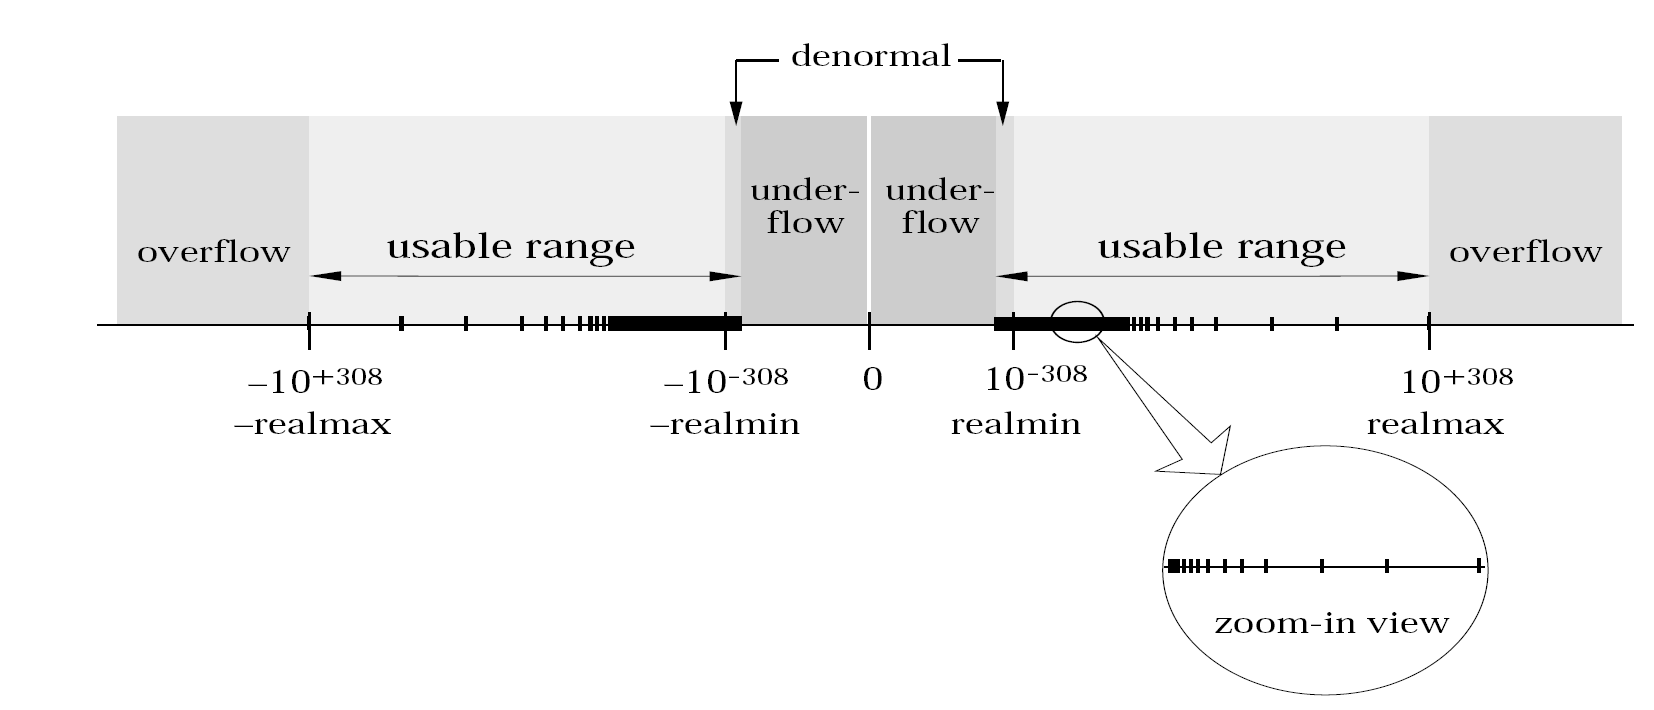
\includegraphics[width=.75\linewidth]{floatingpoints.png}
    \end{center}
\end{document}